%% ID: impulse
%% VIDEO: impulse
%% QUESTIONS: head_on_collusion, what_goes_up
%% LEVEL: 2
%% TOPIC: physics/mechanics/dynamics
%% TYPE: concept
%% TITLE: Impulse
%% ORDER: 150

% This is the template that sets out all of the Problems and produces the Exercise/Solution labels and numbering
% There are two classes of Exercise: "problem" which has a Question and Solution, and "hint" which has a Question, Hint and Solution

% This is the template that sets out all of the Problems and produces the Exercise/Solution labels and numbering
% There are two classes of Exercise: "problem" which has a Question and Solution, and "hint" which has a Question, Hint and Solution

% These are the packages to use in all documents, and the paper size to use:
\documentclass[a4paper,11pt]{article}
\usepackage[usenames,dvipsnames]{xcolor}
\usepackage[margin=1.5cm]{geometry}
\usepackage{amsmath}
\usepackage{amssymb}
\usepackage{color}
\usepackage{graphicx}
\usepackage{graphics}
\usepackage[margin=1.5cm]{geometry}
\usepackage{fancyhdr}
\usepackage{float}
\usepackage{lscape}
\usepackage[font={small},labelfont=bf]{caption}
\usepackage{ifthen}
\usepackage{enumitem}
\usepackage{subcaption}		%Allows grouped figures. The percentage sign after the first \end{subfigure} puts them side by side, omitting it puts one above the other.
\usepackage{graphicx,xcolor} 	%Allows the use of colour in the files
\usepackage{centernot} 		%Puts the / in a not equal to sign in the centre, use as \cnot{...}
\usepackage{comment} 		%Allows \begin{comment} .... \end{comment} to comment out bulk text.
\usepackage{etoolbox}		%Allows the boolean flags and the \toggletrue and \togglefalse commands
\usepackage{cancel}		%Allows the crossing out of terms in maths mode to show they cancel out
\usepackage{wrapfig}

%Packages for font choices
\usepackage{palatino}
\usepackage{mathpazo}


%Then where to find the graphics:
%WARNING -  relative to the TeX file being compiled - NOT this template!
		\graphicspath{{../Diagrams/}{Diagrams/}{./}} %This allows diagrams: {{As a sister folder to Latex}{A subdirectory of LaTeX}{Or just in LaTeX itself}}

% WARNING -  If you want the diagrams to be a sister folder to the LaTeX folder - pdflatex.exe sometimes needs an extra argument to cope with the "../" part; usually it can only cope with subdirectories as opposed to parent ones. If it refuses to compile and says it cannot find the diagrams, either add "--shell-escape" to the start of the arguments of pdflatex, OR move the diagrams to a subdirectory of the one containing the TeX files.
%In TeXworks, to add the extra argument, go to Edit -> Preferences -> Typesetting -> Processing Tools. Click on "pdfLaTeX" -> Edit -> "+" button, then type "--shell-escape" (without quotes) and press the up arrow twice so that it becomes top of the list.


%Then any custom commands written, along with shortcuts and variables:
% This document contains any custom commands, shortcuts and variables needed for the files to compile. It is called by "Problem_Template.tex" and so needs to be in the same directory.

%Defines vectors universally, for ease of editing and consistency.
\newcommand{\vtr}[1] {\mathit{\underline{\boldsymbol{#1}}}}

%Draws a big red box containing the text as in \ALERT{<TEXT HERE>}. For labelling draft copies with important notes.
\def\ALERT#1{\begin{center}\colorbox{red}{\hbox{\textcolor{black}{\textbf{#1}}}}\end{center}}

%Roman-style subscript; removes math-mode font.
\def\s#1{_\textrm{#1} }

%The operators in integrals and derivatives.
\def\d{\operatorname{d}\!}

%The Euler e should be in Roman font.
\def\e{\textrm{e}}

%The Rutherford title, to save typing and for consistency:
\def\Rutherford{Rutherford School Physics}
\def\Concepttitle#1{\noindent\textsc{\Rutherford\vspace{0.4cm}\\ \LARGE Physical Concept: \textbf{#1}}}
\def\Problemtitle#1{\noindent\textsc{\Rutherford\vspace{0.4cm}\\ \LARGE Website Problems: \textbf{#1}}}
\def\AddProblemtitle#1{\noindent\textsc{\Large \Rutherford ~ --- ~ Additional Problems\vspace{0.4cm}\\ \LARGE \textbf{#1}}}
%\def\AddProblemtitle#1{\noindent\textsc{\Rutherford\vspace{0.4cm}\\ \LARGE Additional Problems: \textbf{#1}}}

%define quick question to be used in eg concept sheet.
%\def\qq#2{#1}{\color{red}[#2]\color{black}}
\newcommand{\qq}[2]{\nl Quick Question:\hspace{1 mm} #1\color{red}\hspace{2 mm} Answer:\color{black}\hspace{1 mm}  #2}
\newcommand{\stress}[1]{\emph{#1}}

%%%%%%%%%%%   some definitions used in latexing the CQMP:
% fractions that are of right size in set equations
\def\half{{\textstyle \frac{1}{2}}}
\def\quarter{{\textstyle \frac{1}{4}}}
\def\third{{\textstyle \frac{1}{3}}}
\def\eighth{{\textstyle \frac{1}{8}}}

% obtain a new line
\def\nl{\hfil\break}
\def\nll{\\ \\ \noindent}



%creates numbered lists with a), then i.
\renewcommand{\theenumi}{\alph{enumi}}% first level are latin characters
\renewcommand{\labelenumi}{\theenumi)} %tells it to put a bracket after the character.
\renewcommand{\theenumii}{\roman{enumii}}%second level are little roman characters
\renewcommand{\labelenumii}{\theenumii.} %tells it to put a dot after the character
 % In a file called "Definitions.tex" in the same directory as this file.

%Define some boolean switches:
\newtoggle{solutions_only}	%Print only the solutions
\newtoggle{no_solutions}		%Don't print any solutions  (overridden by solutions_only)
\newtoggle{solutions_at_end}	%Print the solutions at end (overridden by solutions_only and no_solutions)
\newtoggle{no_credits}		%Don't print the credit arguments

%Use this to write a list of things needed to know for a section. It automatically won't print when "solutions_only" is on.
%Its only argument should be a list of things needed to know in "\item [....]" form
\newenvironment{knowledge}[1]{
\iftoggle{solutions_only}{}{It is assumed that students will be familiar with the following concepts:
\begin{itemize} #1 \end{itemize}
\vspace{0.5cm}}
}

%Allows the headings to be managed when not printing problems ect.
\newenvironment{Qsection}[1]{
%\iftoggle{solutions_only}{}{\section{#1}} %Don't output headings in the solutions(?)
\iftoggle{solutions_at_end}{\AtEndDocument{\section{#1}}}{}
\section{#1}
}

\newenvironment{Qsubsection}[1]{
%\iftoggle{solutions_only}{}{\subsection{#1}} %Don't output headings in the solutions(?)
\iftoggle{solutions_at_end}{\AtEndDocument{\subsection{#1}}}{}
\subsection{#1}
}

%Set the values of the boolean switches: Yes - "toggletrue", No - "togglefalse".
\togglefalse{solutions_only}	%	ONLY		Output only solutions? 
\togglefalse{no_solutions}		%	NONE		Don't output solutions at all? 
\togglefalse{solutions_at_end}	%	END		Output solutions at the end?
\togglefalse{no_credits}		%			Don't output the credit field
%All 8 cases have been tested; ONLY takes precedence, then NONE and finally END is lowest.


%##############################################################################################################
%											Then the bulk of the layout options:
%##############################################################################################################

\setlength{\topmargin}{-2cm}
%\setlength{\oddsidemargin}{0.5cm}
%\setlength{\evensidemargin}{0.5cm}


%##############################################################################################################


\newcounter{exercisenumber}%[chapter] %counter is set to zero when "chapter" appears
\def\theexercisenumber{\arabic{exercisenumber}}


\iftoggle{no_solutions}{}{ %Put a header at the end before the solutions, and reset the counter. Only if solutions are being printed AND at the end.
	\iftoggle{solutions_only}{}{
		\iftoggle{solutions_at_end}
			{\AtEndDocument{\newpage \part*{Solutions:} \setcounter{exercisenumber}{0} \setcounter{section}{0}}}{}
	}
}


%%%%%%%%%%%%%%%%%%%%%%%%%%%%%%%%%%%%%%%%%%%%%%%%%%%%%%%%%%%%%%%%%%%%%%%%%%%%%%%%%
%Creates \begin{problem}[label]{exercise_text}{source_text}{solution_text}\end{problem} command - the label argument is optional
%If put in, remember to put in [] brackets.  A label called label.ex will be generated.
\newenvironment{problem}[4][noref]{
 \refstepcounter{exercisenumber} %\refstepcounter allows you to reference to the exercise number
%
\iftoggle{solutions_only}{\hfil\break \textit{Solution}~\theexercisenumber:  #4}{ %If only solutions, just output solution.
	\noindent{\textit{Exercise}~\theexercisenumber:}
	\ifthenelse{\equal{#1}{noref}}{}{\label{#1.ex}} #2 %\vspace{0.3cm}
	\iftoggle{no_credits}{}{
			%\hfil\break {\small #3} \vspace{0.3cm} %This is the old line, replaced with the one below, without the ifthenelse statement; in case something goes wrong.
			\ifthenelse{\equal{#3}{}}{}{ {\tiny [#3]} \vspace{0.3cm}} %If the credit field is blank; don't bother printing it or the space for it.
	} %reference argument
%
	\iftoggle{no_solutions}{}{ %If the solutions aren't to be printed, do nothing.
		\iftoggle{solutions_at_end}
			{\AtEndDocument{\stepcounter{exercisenumber}\hfil\break \textit{Solution}~\theexercisenumber:  #4 \vspace{0.5cm}}} %If at the end: do this.
			{\hfil\break \textit{Solution}~\theexercisenumber:  #4} 	%Else leave in line as in TeX file.
	}
}

\vspace{0.2cm}}

%%%%%%%%%%%%%%%%%%%%%%%%%%%%%%%%%%%%%%%%%%%%%%%%%%%%%%%%%%%%%%%%%%%%%%%%%%%%%%%%%
%Creates \begin{hint}[label]{exercise_text}{hint_text}{source_text}{solution_text}\end{hint} command - the label argument is optional
%If put in, remember to put in [] brackets.  A label called label.ex will be generated.
\newenvironment{hint}[5][noref]{
 \refstepcounter{exercisenumber}
%
\iftoggle{solutions_only}{\hfil\break \textit{Solution}~\theexercisenumber:  #5}{  %If only solutions, just output solution.
	\noindent{\textit{Exercise}~\theexercisenumber:}
	\ifthenelse{\equal{#1}{noref}}{}{\label{#1.ex}} #2 \vspace{0.1cm}
	 \hfil\break  \textit{Hint:}  #3{} %\vspace{0.3cm}
	\iftoggle{no_credits}{}{
			\ifthenelse{\equal{#4}{}}{}{\\ \hfil {\tiny #4} \vspace{0.3cm}} %This is the old line, replaced with the one below, without the ifthenelse statement; in case something goes wrong.
			%\ifthenelse{\equal{#4}{}}{}{{\tiny [#4]} \vspace{0.3cm}} %If the credit field is blank; don't bother printing it or the space for it.
	} %reference argument
%
	\iftoggle{no_solutions}{}{%If the solutions aren't to be printed, do nothing.
		\iftoggle{solutions_at_end}
			{\AtEndDocument{\stepcounter{exercisenumber}\hfil\break \textit{Solution}~\theexercisenumber:  #5 \vspace{0.5cm}}} %If at the end: do this.
			{\hfil\break \textit{Solution}~\theexercisenumber:  #5}%Else leave in line as in teX file.
	}
}
\vspace{0.2cm}}

%%%%%%%%%%%%%%%%%%%%%%%%%%%%%%%%%%%%%%%%%%%%%%%%%%%%%%%%%%%%%%%%%%%%%%%%%%%%%%%%%


 %%%%%%%
\newenvironment{additional}[2][noref]{
 \refstepcounter{exercisenumber}
% \vspace{.2cm}
\nl
\noindent{\textit{Exercise}~\theexercisenumber:}
\ifthenelse{\equal{#1}{noref}}{}{\label{#1.ex}} #2 }{%\vspace{5.1cm}
 }
%










%*******************************
% to mark as a draft.  Comment both these lines out when complete.  The page number will return to the footer.
%\pagestyle{myheadings}
%\markright{\textcolor{red}{\textbf{DRAFT: \today}}}


\begin{document}
\addtolength{\topmargin}{-0.7 cm}
\setlength{\columnsep}{22pt}
\Concepttitle{Impulse}


\section{What is impulse?}
When Newton described his second law of motion he said that an impulse causes a change in momentum in the direction that the impulse is applied.  We often find it useful to discuss this law in terms of a resultant force and the rate of change of momentum (or for constant mass ${\vtr  F}=m{\vtr a}$) but thinking in terms of an impulse allows us to take into account the length of time for which the force is applied.\\

\begin{wrapfigure}{r}{7cm}
\center
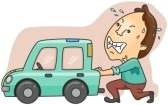
\includegraphics[width=0.3\textwidth]{figures/Impulse1.eps}
\caption{How does the final speed of a broken down car change if you apply the same force for different lengths of time?}\vspace{1.0cm}
\end{wrapfigure} 

\noindent If we think about some real physical situations, our intuition tells us that if we apply a force to an object for longer, its final velocity will be greater.  Imagine trying to push start a car.  If the car is at rest and you begin pushing with a constant force, then the longer you keep pushing, the faster the car will be moving when you let go.\\

\noindent The definition or formula to calculate an impulse is simply,
\begin{equation}
{\vtr I}={\vtr F}{t}.
\end {equation}
As force is a vector quantity so must the impulse be a vector; Newton's second law hints at this because he tells us that it is important to consider the direction in which the impulse was applied.


\section{But what does it mean?}
This formula does not give us much of a sense of what impulse {\it actually} is or what it means.  Let's go back to the idea that Newton describes in his second law of motion that {\it an applied impulse acts to change the momentum of a body in the direction that the impulse is applied}.\\

\begin{wrapfigure}{r}{7cm} 
\center
\includegraphics[width=0.3\textwidth]{figures/Momentum1.eps}
\caption{The graph of a constant force of $10$ N applied to an object for $5$ seconds.  The impulse that the object experiences is ${\vtr F}t = 50$ Ns which is also given by the area under the line of the graph, shown in pink.}\label{impulse1}
\end{wrapfigure}

\noindent When we apply an impulse to something our intuition tells us that it will change from being at rest to moving with some speed in the direction that we applied the impulse.  By applying an impulse we will change its momentum from zero to some value given by its mass times its velocity and we would guess that the larger the impulse the greater the change in momentum.

\subsection*{Levels 1-4}
If a constant force is applied to a body for a given time then the impulse is the vector quantity given by
\begin{equation} \label{imp1}
\mbox{\bf Impulse} = \vtr{I} = \mbox{\bf force} \times \mbox{time} ={\vtr F}t
\end{equation}
This relationship (equation \ref{imp1}) shows that we can increase the magnitude of the impulse by either increasing the magnitude of the force or increasing the amount of time over which we apply the force.\\

\noindent So following Newton's Law,
\begin{eqnarray}
\mbox{Impulse}&=&\mbox{change in momentum}\nonumber \\
&=&\mbox{final momentum} - \mbox{initial momentum}\nonumber \\
{\vtr F}t &=& m{\vtr v}-m{\vtr u} = m({\vtr v}-{\vtr u})
\end{eqnarray}
where $m$ is the mass of the body, ${\vtr v}$ is the final velocity of the body after we have applied the impulse, ${\vtr u}$ is the initial velocity of the body, ${\vtr F}$ is the force that we apply and $t$ is the time over which we apply the force.\\

\noindent We can now see the connection to Newton's Second Law as we learn it at school if we do a little rearrangement of our formula,
\begin{eqnarray}
{\vtr F}t&=&m({\vtr v}-{\vtr u})\nonumber \\
{\vtr F}&=&m\frac{({\vtr v}-{\vtr u})}{t}
\end{eqnarray}

\noindent A change in velocity $(v-u)$ divided by the time it takes for that change $t$ is the average acceleration of the body, so
\begin{equation}
{\vtr F}=m{\vtr a}
\end{equation}


\subsection*{Quick Questions}
\begin{itemize}
\item[1.] A broken down car of $1000$\ kg is pushed with a force of $50$ N for $2$ minutes.  If we neglect friction, what speed would the car finally reach? \color{red}[$v=6$ ms$^{-1}=21.6$ kph$=13.5$ mph]\color{black}
\item[2.] What force does a netball player apply to a ball of mass, $500$ g, when she catches it from her team-mate if the ball is travelling at $5$ ms$^{-1}$ and it takes her $0.1$ s to catch it?  How could she reduce the amount of force that she needs to apply? \color{red}[${\vtr F}=-25$ N, i.e. the force is in the opposite direction to the motion of the ball.]\color{black}
\item[3.] A perfectly hard air hockey puck of $50$ g, is travelling towards you at $10$ ms$^{-1}$ and you want to send it back to your opponent at $15$ m$s^{-1}$.  Your bat will be in contact with the puck for $0.01$ s, what force do you need to apply to the puck? \color{red}[${\vtr F}=-125$ N, i.e. the force is in the opposite direction to the initial motion and in the direction back towards your opponent.] \color{black}
\item[4.] In July 2011 a baby fell 10 stories from a hotel window and was caught by a passer-by and they both survived (http://www.bbc.co.uk/news/magazine-14150524).  If the force that the catcher experienced was $30$ kN over a period of $0.02$ s, how fast was the baby falling just before the catch happened (we estimate the mass of the baby as $10$ kg)? \color{red}[$u=60$ ms$^{-1}$ downwards.]\color{black}
\item[5.] A squash ball, of mass $25$ g, rebounds off a wall at $60$ ms$^{-1}$ and the wall exerts an force of $300$ N for a period of $10$ ms.  How fast is the ball going when it first collides with the wall?  Is your answer physically possible? If not why not? \color{red}[$u=60$  ms$^{-1}$ towards the wall.  This is not physically possible because in reality the collision will not be elastic.]\color{black}
\end{itemize}

\subsection*{Level 5 +}
The simplest case, in which we can calculate an impulse, is where a constant force is applied to a body for an amount of time $t$ (as shown in figure \ref{impulse1}) but we might also want to consider situations where the strength of the force varies in time (figure \ref{impulse2}).  If the force is not constant with time then we need to calculate the total impulse applied over a given time interval to calculate the total change in momentum.  This total impulse is again equal to the area under the force-time graph.

\noindent The geometry in our example is reasonably simple (figure \ref{impulse2}) so we can use the area of a triangle subtracted from the area of a rectangle to work this area out.
\begin{eqnarray}
Area = {\vtr I} &=&  {\vtr F_f}t_f-\frac{({\vtr F_f}-{\vtr F_i})t_f}{2} \nonumber \\
{\vtr I}&=&\frac{({\vtr F_f}+{\vtr F_i})t_f}{2} \label{area_tri}
\end{eqnarray}

\begin{wrapfigure}{r}{7cm} 
\center
\includegraphics[width=0.3\textwidth]{figures/Momentum2.eps}
\caption{The graph of a force that changes over time from an initial value of $F_i$ N  to $F_f $ N over a time of $t$ seconds.  The impulse that the object experiences can be calculated using the area under the line of graph, shown in pink.}  \label{impulse2}
\end{wrapfigure} 
\noindent But we can also use this force-time graph to illustrate how we would calculate the impulse in a general case, when the area cannot be simply expressed because the force-time relationship is more complex.\\

\noindent We can calculate the area under the force line by adding up the areas of a series of small rectangles of width $\d t$ from $t=0$ to $t=t_f$. Using figure \ref{impulse2} we can see that the area of a small rectangle is given by the height of the rectangle ${\vtr F}$ multiplied by the width of the rectangle $\d t$.  The instantaneous impulse, $\d{\vtr I}$ at time $t$ is therefore
\begin{equation}
\d{\vtr I} = {\vtr F}\d t
\end{equation}
The force-time graph in figure \ref{impulse2} shows that the force varies with time as a straight line, so ${\vtr F}=kt+c$, where the gradient of the line 
\begin{equation}
k=\frac{({\vtr F_f}-{\vtr F_i})}{t_f}
\end{equation}
and the vertical intercept $c={\vtr F_i}$, so therefore the force at any given time is.
\begin{equation}
{\vtr F}=\frac{({\vtr F_f}-{\vtr F_i})t}{t_f}+{\vtr F_i}
\end{equation}

\noindent To find the total impulse we need to add up all the small areas which we can do by integrating this equation for the force over time.
\begin{eqnarray}
{\vtr I}&=&\int_0^{t_f}{{\vtr F} \d t}\nonumber \\
&=&\int_0^{t_f}\left[\frac{({\vtr F_f}-{\vtr F_i})t}{t_f}+{\vtr F_i}\right] \d t\nonumber\\
{\vtr I}&=&\left[\frac{({\vtr F_f}-{\vtr F_i})t^2}{2t_f}+{\vtr F_i}t\right]_0^{t_f}\nonumber\\
{\vtr I}&=&\frac{({\vtr F_f}-{\vtr F_i})t_f}{2}+{\vtr F_i}t_f\nonumber\\
{\vtr I}&=&\frac{({\vtr F_f}+{\vtr F_i})t_f}{2}
\end{eqnarray}
We can see, therefore, that integrating the equation for the force over time produces the same result as calculating the area under the graph by triangles given by equation \ref{area_tri}.

\subsection*{Quite Quick Questions}
\begin{itemize}
\item[1.] An impulse is applied to a ball of mass, $500$ g, according to the force-time relation shown in figure \ref{impulse2}  in the same direction as its initial velocity.  What is the final velocity of the ball if it has an initial velocity of $10$ ms$^{-1}$ and the parameters of the force-time graph are, $t_f=1$ s, $F_i=5$ N and $F_f=10$ N. \color{red}[$v=25$ ms$^{-1}$ in the direction of motion.] \color{black}
\item[2.] A pram complete with baby ($20$ kg) is left $1$ km up along a straight path from the bottom of a hill which is inclined at $30^\circ$ to the horizontal. The pram's brakes fail and the pram begins to perfectly roll down the hill under gravity.   What impulse will be required to stop the pram at the bottom of the hill? [Let the acceleration due to gravity, $g=10$ ms$^{-2}$]. \color{red}[$I=2000$ Ns in the direction opposite to the motion of the pram]\color{black}
\item[3.] A pinball table uses a compressed spring, with spring constant $k$, to accelerate a steel ball of mass $m$, from rest to as high a speed as possible.   Hooke's Law tells us that the force exerted by the spring depends on the extension, $x$ of the spring;
\begin{equation}
{\vtr F}=-k{\vtr x} \nonumber
\end{equation}
and the extension of the spring in our example will change with time as $x=A\cos(\omega t)$.  Write down the integral expression for the impulse over the interval $t=0$ to $t'$ that would allow us to calculate the velocity of the ball when it leaves the spring at time $t'$. Using this expression what is the velocity of the steel ball after a time, $t'$.\color{red}\begin{equation}[v=\frac{-kA}{m}\int_0^{t'} \cos(\omega t) \d t\nonumber\end{equation} \begin{equation}v=\frac{kA\sin(\omega t')}{m\omega}]\nonumber\end{equation}

\end{itemize}
\end{document}
